% Created 2016-04-11 Mon 01:56
% Intended LaTeX compiler: pdflatex
\documentclass[11pt]{article}
\usepackage[utf8]{inputenc}
\usepackage[T1]{fontenc}
\usepackage{graphicx}
\usepackage{grffile}
\usepackage{longtable}
\usepackage{wrapfig}
\usepackage{rotating}
\usepackage[normalem]{ulem}
\usepackage{amsmath}
\usepackage{textcomp}
\usepackage{amssymb}
\usepackage{capt-of}
\usepackage{hyperref}
\usepackage{minted}
\usepackage[margin=0.75in]{geometry}
\newcommand{\norm}[1]{\Vert #1 \Vert}
\newcommand{\opnorm}[1]{\Vert #1 \Vert_{op}}
\newcommand{\fnorm}[1]{\Vert #1 \Vert_F}
\newcommand{\nucnorm}[1]{\Vert #1 \Vert_*}
\newcommand{\tr}{\operatorname{Tr}}
\newtheorem{theorem}{Theorem}[section]
\newtheorem{lemma}[theorem]{Lemma}
\newtheorem{proposition}[theorem]{Proposition}
\newtheorem{corollary}[theorem]{Corollary}
\newtheorem{proof}[theorem]{Proof}
\author{Bachir El khadir}
\date{\textit{<2016-04-02 Sat>}}
\title{Problem set 5, ORF523}
\hypersetup{
 pdfauthor={Bachir El khadir},
 pdftitle={Problem set 5, ORF523},
 pdfkeywords={},
 pdfsubject={},
 pdfcreator={Emacs 25.1.50.1 (Org mode )}, 
 pdflang={English}}
\begin{document}

\maketitle


\section{Problem 1}
\label{sec:orgheadline1}


Notation \(E_{ij} = (\delta_{ik}\delta_{jl} + \delta_{il}\delta_{jk})_{k,l}\) the matrix with all 0 except in \((i, j)\) and \((j, i)\)


\begin{align*}
-\nu(G) =
& \underset{X}{\text{min}}
& & Tr(X(-J)) \\
& \text{subject to}
& & X \ge 0
\\&&& Tr(XI_n) = 1 &(:& \alpha)
\\&&&Tr(E_{ij}X) = 0 \; \forall (i,j) \in E, i < j &(:& \lambda_{ij})
\end{align*}

has  for dual:

\begin{align*}
& \underset{\alpha, \lambda_{ij} \in \mathbb R}{\text{max}}
& & \alpha \\
& \text{subject to}
& & \alpha I + \sum_{(i,j) \in E} \lambda_{ij} E_{ij} \le -J
\end{align*}
Or:

\begin{align*}
& \underset{\alpha, \lambda_{ij} \in \mathbb R}{\text{max}}
& & \alpha \\
& \text{subject to}
& & \alpha I + \sum_{(i,j) \in E, i < j} \lambda_{ij} E_{ij} \le -J
\end{align*}


Both are strictly feasible:
\begin{itemize}
\item for the primal, take \(X = \frac{I_n}n\)
\item For the dual, take \(\alpha = -2\), \(\lambda_{ij} = 0\)
\end{itemize}
Which proves that the dual and primal are equal. Taking  \(\beta = -\alpha\), we can write that:



\begin{align*}
\nu(G) = 
& \underset{\alpha, \lambda_{ij} \in \mathbb R}{\text{min}}
& & \beta \\
& \text{subject to}
& & -\beta I + \sum_{(i,j) \in E} \lambda_{ij} E_{ij} \le -J
\end{align*}
Note that the \((1, 1)\) entry of \(-\beta I + \sum_{(i,j) \in E} \lambda_{ij} E_{ij} + J\): \(1-\beta\) shoud be negative, so we can ammend to the constraints that \(\beta \ge 1\)

\begin{align*}
-\beta I + \sum_{(i,j) \in E} \lambda_{ij} E_{ij} \le -J
&\iff \beta(I - \sum_{(i,j) \in E} \frac{\lambda_{ij}}{\beta} E_{ij}) \ge J
\\&\iff I - \sum_{(i,j) \in E} \frac{\lambda_{ij}}{\beta} E_{ij}) \ge \frac1\beta 11^T
\\&\iff \begin{pmatrix}I - \sum_{(i,j) \in E} \frac{\lambda_{ij}}{\beta} E_{ij} & \begin{matrix}1\\\vdots\\1\end{matrix}\\
 \begin{matrix}1&\ldots&1\end{matrix}&\beta\end{pmatrix} \ge 0 &\text{(By Schur Lemma bc $\beta > 0$)}
\end{align*}


Let's note this big matrix \(Z\). It is clear that a matrix \(Z \in S^{(n+1) \otimes (n+1)}\) is of this form iff it verifies the constraints of the following optimization problem:
\begin{align*}
& \underset{\alpha, \lambda_{ij} \in \mathbb R}{\text{min}}
& & Z_{n+1, n+1} \\
& \text{subject to}
& & Z \ge 0
\\&&& Z_{i,n+1} = Z_{ii} = 0
\\&&& Z_{i,j} = 0 \forall \{i, j\} \in \bar E
\end{align*}

Which is then equal to \(\vartheta(G)\)

Let \(C = \chi(\bar G)\)
By definition, there exist a partition of \(V\): \(\{V_1, \ldots, V_C\}\) such that \(V_i\) is a clique for all \(i \le C\)
\begin{itemize}
\item Define \(1_{V_i} \in \mathbb R^n\) to be the indicator function of the set \(V_i\), and note that \(1 = \sum_{i \le C} V_i\)
\item Define \(z_i = \begin{pmatrix}1_{V_i}\\1\end{pmatrix} \in \mathbb R^{n+1}\). Note that:
$$z_iz_i^T = \begin{pmatrix}1_{V_i}1_{V_i}^T&1_{V_i}\\1^T_{V_i}&1\end{pmatrix}$$
\item Define $$Z = \sum_{i} z_iz_i^T = \begin{pmatrix}\sum 1_{V_i}1_{V_i}^T&1\\1^T&C\end{pmatrix}$$. \(Z\) is positive semidefinite because it is a sum of psd terms \(z_iz_i^T\)
\item \((1_{V_i}1_{V_i}^T)_{kl} = (e_k^T1_{V_i})(e_l^T1_{V_i}) = 1_{V_i}(k) 1_{V_i}(l)\). If \((k, l) \in \bar E\), then the \(k^{th}\) node and the \(j^{th}\) node cannot be in the same \(V_i\), and therfore \((1_{V_i}1_{V_i}^T)_{kl} = 0\)
\item If \(k = l\), all the terms in \(\sum_i (1_{V_i}1_{V_i}^T)_{kl}\) are zero except for the \(i\) for which the \(k^{th}\) node is in \(V_i\), in which case it is equal to one.
\end{itemize}

As a conclusion, \(Z\) verifies all constraints of the dual, and \(Z_{n+1, n+1} = C = \chi(\bar G)\), so $$\chi(\bar G) \ge \vartheta(G)$$


\textbf{2}

Consider \(G = C_5\).

Using CVX to calculate \(\vartheta(G)\)
\begin{minted}[frame=lines,linenos=true]{matlab}
n = 5
J = ones(n, n);
cvx_begin sdp
variable X(n, n) symmetric;
maximize(trace(X*J))
X >= 0
X(5, 1) == 0
for i=1:4
    X(i, i+1) == 0
end
trace(X) == 1
cvx_end
ans=cvx_optval
\end{minted}

\begin{verbatim}
2.2361
\end{verbatim}


\(2 < \vartheta(G) < 3\)

\begin{itemize}
\item \(\vartheta(G) \not \in \mathbb N\)
\item \(\alpha(G), \chi(\bar G) \in \mathbb N\)

No inequality can thus be tight.
\end{itemize}

\section{Q2}
\label{sec:orgheadline4}

\textbf{1}
-------------Duality---------------

Let \(x \in [0, 1]^n\) such that \(C_1, \ldots C_k\)

Consider
\[Y = \begin{pmatrix}
x_1 & \hfill & \hfill & \hfill & x_1 \\
\hfill & x_2 & \hfill & 0 & x_2 \\
\hfill & \hfill & \ddots &\hfill & \vdots \\
\hfill & 0 & \hfill & x_n & x_n \\
x_1 & x_2 & \ldots & x_n & 1 \\
\end{pmatrix}\]




\textbf{2}
\begin{org}
\begin{center}
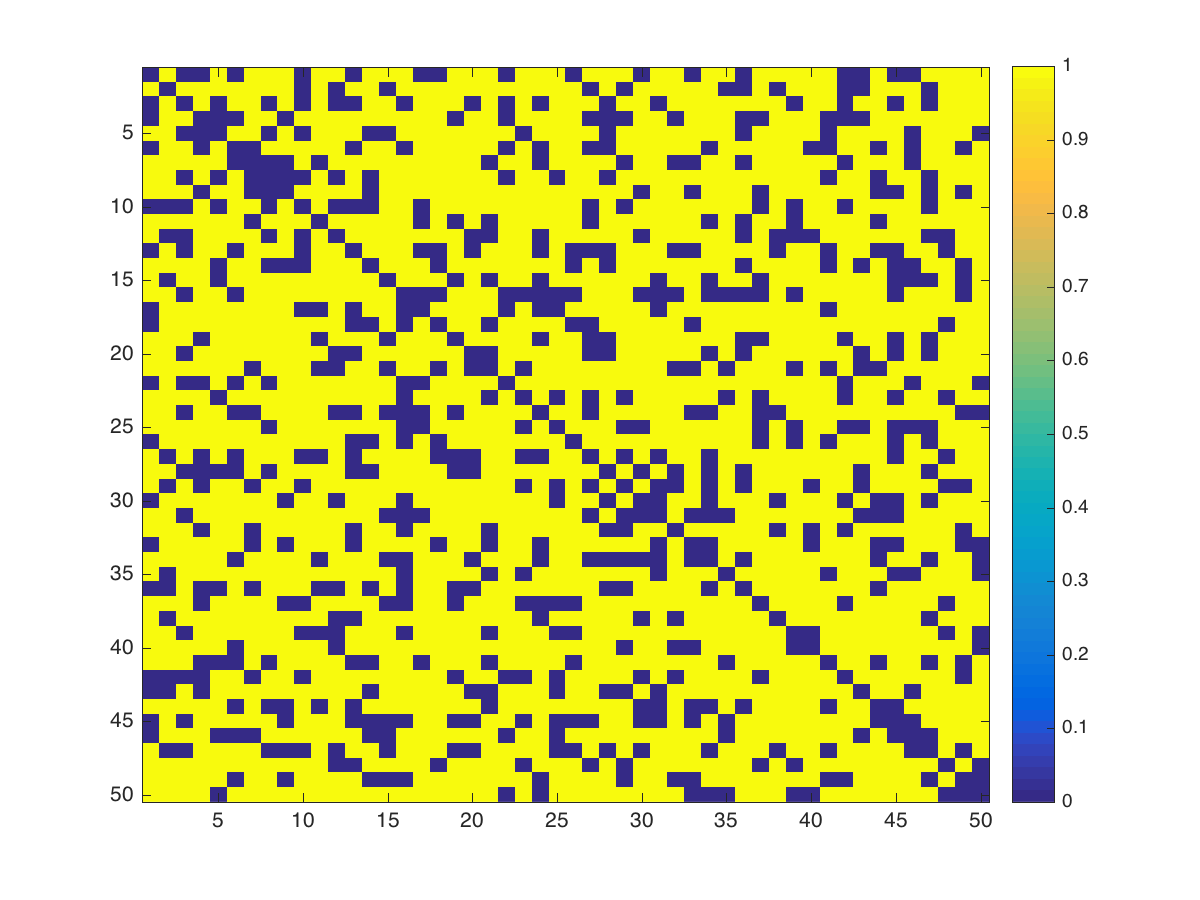
\includegraphics[width=0.35\textwidth]{graph.png}
\captionof{figure}{G Adjacency matrix}
\end{center}
\end{org}




\subsection{\(\vartheta(G)\)}
\label{sec:orgheadline2}
\begin{minted}[frame=lines,linenos=true]{matlab}
n = 50
J = ones(n, n);

cvx_begin sdp
variable X(n, n) symmetric;
maximize(trace(X*J))
X >= 0
for i=1:n
    for j=1:i
        if G(i, j) == 1
            X(i, j) == 0
        end
    end
end
trace(X) == 1
cvx_end

ans=cvx_optval
\end{minted}

\begin{verbatim}
5
\end{verbatim}










\begin{org}
\begin{center}
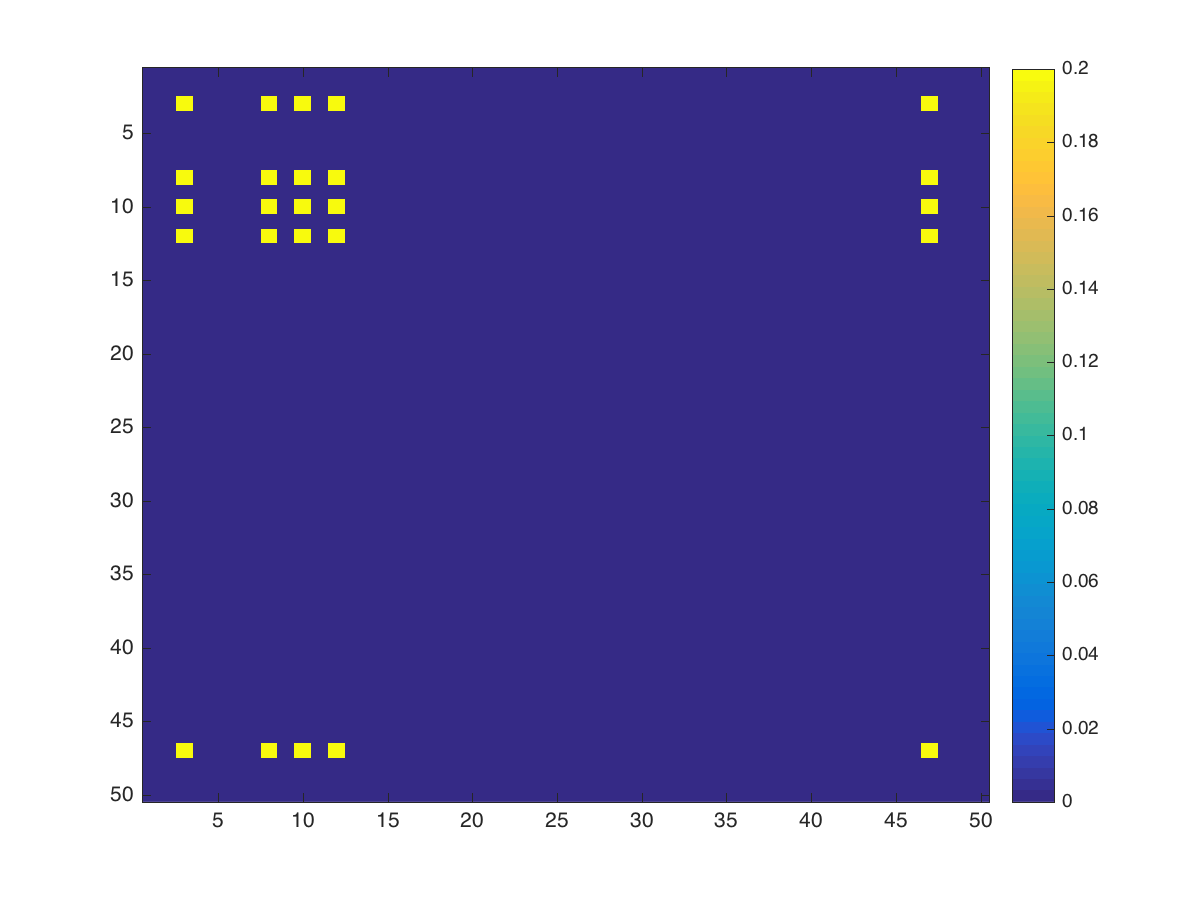
\includegraphics[width=0.35\textwidth]{X.png}
\captionof{figure}{X optimal solution}
\end{center}
\end{org}




Note that the resulting \(X\) is of rank 1, so it can be decomposed into \(X = xx^T\). We check that \(V_x = \{i , x_i \ne 0\}\) represents indeed a stable set.
\begin{minted}[frame=lines,linenos=true]{matlab}
[v,e] = eigs(full(X),1);
stableset = find(abs(v) > 0.01)  
ans=stableset'
\end{minted}

\begin{center}
\begin{tabular}{rrrrr}
3 & 8 & 10 & 12 & 47\\
\end{tabular}
\end{center}


\begin{minted}[frame=lines,linenos=true]{matlab}
G(stableset, stableset)
\end{minted}

\begin{org}
\begin{center}
\captionof{table}{Subgraph of the nodes in the stableset}
\begin{tabular}{rrrrr}
0 & 0 & 0 & 0 & 0\\
0 & 0 & 0 & 0 & 0\\
0 & 0 & 0 & 0 & 0\\
0 & 0 & 0 & 0 & 0\\
0 & 0 & 0 & 0 & 0\\
\end{tabular}
\end{center}
\end{org}


Let's assume that there exist another stable set of size 5 \(V_y\).

This would mean that there exist \(v \in V_x\) such that imposing \(X_{jj} = 0\) would not change \(\alpha\). Let's check:

\begin{minted}[frame=lines,linenos=true]{matlab}
  n = 50
  J = ones(n, n);
  opt = [stableset, zeros(5, 1)]
  for vi=1:5
      v = stableset(vi)
      cvx_begin sdp
      variable Y(n, n) symmetric;
      variable optvalue;
      maximize(trace(Y*J))
      Y >= 0
      for i=1:n
          for j=1:i
              if G(i, j) == 1
                  Y(i, j) == 0
              end
          end
      end
      Y(v,v) == 0
      trace(Y) == 1
      optvalue == trace(Y*J)
      cvx_end
      opt(vi, 2) = optvalue
  end
ans=opt
\end{minted}

\begin{org}
\begin{center}
\captionof{table}{Lovazs}
\begin{tabular}{rr}
Node removed & Lovasz of the subgraph\\
\hline
3 & 4.4463\\
8 & 4.5191\\
10 & 4.512\\
12 & 4.5586\\
47 & 4.4771\\
\end{tabular}
\end{center}
\end{org}



Since Lovasz number \(\vartheta\) is an upper bound on \(\alpha\), This proves that any stable set not containing one of the nodes in \(V_x\) is of size less than \(5\).

We have just proved uniqueness of the stable set.

\subsection{\(\mu^{LP}\)}
\label{sec:orgheadline3}

k = 2

\begin{minted}[frame=lines,linenos=true]{matlab}
cvx_begin 
variable x(n)
maximize(sum(x))
for i=2:n
    for j=1:(i-1)
        if G(i, j) == 1
            x(i) + x(j) <= 1
        end
    end
end
0 <= x <= 1
cvx_end

ans=cvx_optval
\end{minted}

\begin{verbatim}
25
\end{verbatim}


k = 3

\begin{minted}[frame=lines,linenos=true]{matlab}
cvx_begin 
variable x(n)
maximize(sum(x))
for i=2:n
    for j=1:(i-1)
        if G(i, j) == 1
            x(i) + x(j) <= 1
        end
        for r=1:(j-1)
            if G(i, j) +  G(j, r) + G(r, i) == 3
                x(i) + x(j) + x(r) <= 1
            end
        end
    end
end
0 <= x <= 1
cvx_end

ans=cvx_optval
\end{minted}

\begin{verbatim}
16.667
\end{verbatim}

k = 4
\begin{minted}[frame=lines,linenos=true]{matlab}
M = 50
cvx_begin 
  variable x(n)
  maximize(sum(x))
  for i=2:M
      for j=1:(i-1)
          if G(i, j) == 0
              continue
          end
          x(i) + x(j) <= 1
          for r=1:(j-1)
              if G(j, r) == 0 || G(r, i) == 0
                  continue
              end
              x(i) + x(j) + x(r) <= 1
              for p =1:(r-1)
                  if G(i, p) == 0 || G(j, p) == 0 || G(r, p) == 0
                      continue
                  end
                  x(i) + x(j) + x(r) + x(p) <= 1
              end
          end
      end
  end
  0 <= x <= 1
  cvx_end

  ans=cvx_optval
\end{minted}

\begin{verbatim}
12.5
\end{verbatim}




\section{Problem 3}
\label{sec:orgheadline5}
\textbf{1.}
Let \((a, b), (u, v)\) be two nodes in \(G_A \otimes G_B\)
The two nodes are connected if and only if:
\begin{itemize}
\item \(A_{au} = 1, A_{bv} = 1\)
\item \(a = u, A_{bv} = 1\)
\item \(A_{au} = 1, b = v\)
\end{itemize}
This can be summerised as \((A_{au} + \delta_{au})(A_{bv} + \delta_{bv}) - \delta_{au}\delta_{bv} = 1\)

So the adjacency matrix of \(G_A \otimes G_B\) is \((A+I_{n}) \otimes (B+I_m) - I_{nm}\).

Where \(\otimes\) denote the Kronecker product: \((A\otimes B)_{p(r-1)+v, q(s-1)+w} = A_{rs} B_{vw}\)

\textbf{2.}




\section{Problem 4}
\label{sec:orgheadline6}

\textbf{1.}
(1) is equivalent to
\[\left\{\begin{array}{cc}
  x^TAy &= \max_{\tilde x \in \Delta_m} \tilde x^TAy\\
  x^TBy &= \max_{\tilde y \in \Delta_n}  x^TB\tilde y
  \end{array}\right.\]

Consider the first problem:
$$\max_{\tilde x \in \Delta_m} \tilde x^TAy$$

This is an LP whose feasible region   \(\Delta_m = conv(e_i, i=1\ldots m)\) is compact, so the maximum is attained in one of the extreme points \(e_{i_0}\). Therefore 

$$x^TAy = \max_{\tilde x \in \Delta_m} \tilde x^TAy \iff x^TAy = e_{i_0}^TAy = \max_{i} e_i^TAy \iff x^TAy \ge e_i^TAy \forall i$$
Same argument applies for \(y\) so that:
$$x^TBy = \max_{\tilde y \in \Delta_n} x^TB \tilde y  \iff x^TAy \ge x^TBe_i \forall i$$

So: \[(1) \iff \left\{\begin{array}{cc}
  x^TAy &\ge e_i^TAy \; \forall i = 1\ldots m\\
  x^TBy &\ge x^TAe_i \; \forall i = 1\ldots n
  \end{array}\right.\]

\textbf{2.}

\(x \in \Delta_m, y \in \Delta_n\)

Note \(z = \begin{pmatrix}x \\ y\end{pmatrix}, u = \begin{pmatrix}1 \\ 0\end{pmatrix}, v = \begin{pmatrix}0 \\ 1\end{pmatrix}\), 
\(M = zz^T = \begin{pmatrix}xx^T&xy^T\\yx^T&yy^T\end{pmatrix}\)

Note that
\begin{itemize}
\item \(M \succeq 0\)
\item \(rank(M) = 1\)
\item \(u^TMu = 1^Txx^T1 = (1^Tx)^2 = 1\), similarly \(v^TMv = 1\)
\item \(M_{(i+m), j} = x_iy_j \ge 0\)
\end{itemize}

Now let \(M \in S^{n+m}\), verifying all the previous conditions. Then by cholesky, there existe a vector \(z \in \mathbb R^{n+m}\), such that: \(M = zz^T\)

\begin{itemize}
\item Let's decompose \(z := \begin{pmatrix}x \\ y\end{pmatrix}\)
\item \(1 = u^TMu \implies \sum_i x_i = \pm 1\), similarly, \(\sum y_j = \pm 1\)
\item \(M_{(i+m), j} = x_iy_j \ge 0 \implies x_i, y_j\) all share the same sign.
\item We can always change \(x\) and/or \(y\) to \(-x, -y\) to make \(x, y \ge 0\) and therefore \(\sum_i x_i = \sum_j y_j = 1\), e.g \(x \in \Delta_m, y \in \Delta_n\)
\item \(Mu = \begin{pmatrix}xx^T 1\\yx^T1\end{pmatrix} = \begin{pmatrix}(x^T 1) x\\(x^T1)y\end{pmatrix} = \begin{pmatrix}x\\y\end{pmatrix}\)
\item \(x = \underbrace{\begin{pmatrix}I_n&0\\0&0\end{pmatrix}}_{J_1}Mu\)
\item \(y = \underbrace{\begin{pmatrix}0&0\\0&I_m\end{pmatrix}}_{J_2}Mu\)
\item \(yx^T = M_{n:n+m, 1:n}\)
\end{itemize}

The constraint of \((2)\) can be formulated as follow:

\begin{itemize}
\item $$x^TAy = tr(yx^TA) = tr(M_{n:n+m, 1:n} A)$$
\item \(e_i^TAy = e_i^TAJ_2Mu = tr(ue_i^T AJ_2 M)\)
\item \(x^TBy = tr(M_{n:n+m, 1:n} B)\)
\item \(x^TBe_i = (J_1Mu)^TBe_i = u^TMJ_1Be_i = tr(M J_1Be_iu^T)\)
\end{itemize}

In conclusion:
\begin{itemize}
\item \(M \succeq 0\)
\item \(rank(M) = 1\)
\item \(M_{i+m, j} \ge 0\)
\item \(tr(M uu^T) = 1\)
\item \(tr(M_{n:n+m, 1:n} A) \ge tr(M ue_i^TAJ_2)\)
\item \(tr(M_{n:n+m, 1:n} B) \ge tr(M J_1Be_iu^T)\)
\end{itemize}
\end{document}